\chapter{Implementation}
\section{Tech Stack Justification}
\section{Backend Architecture}
\section{Frontend Interface and Features}

\begin{figure}[h]
    \centering
    \fbox{
    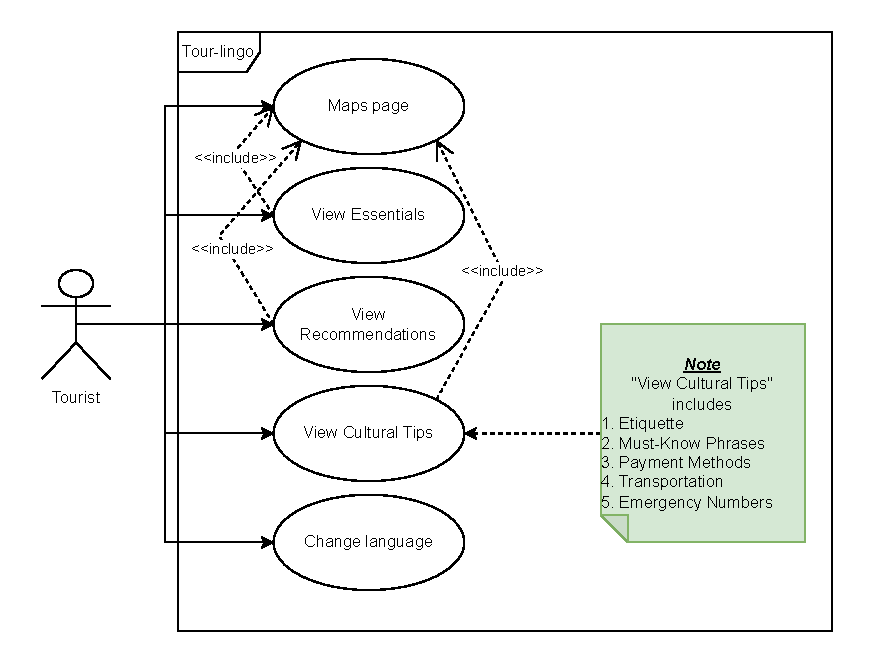
\includegraphics[width=0.5\linewidth]{chapter/05_implementation/Frontend_Usecase_Diagram.pdf}
    }
    \caption{Frontend Usecase Diagram}
    \label{fig:frontend_usecase}
\end{figure}

\section{API and Integration}
\subsection{Drafting notes}

Stuff that is relevant to include here + the ideas of what/how to do this from other reports + the common theme to have there
\begin{itemize}
    \item I guess the project should be written in a very casual style, with plain English and for the reader that may have a very limited understanding of how to use the software engineering tool and services.
    \item To be honest, it seems like I can just list the API's that we use, discuss their pros and cons in the context of the alternatives and explain briefly how they work/what they do. Maybe draw some diagrams and insert them here. Can do in that motivation/methods/discussion way, but we'll see how that goes.
\end{itemize}

Okay, which API's/third party software and services do we actually use:
\begin{itemize}
    \item The main page
    \begin{itemize}
        \item This zustand thing
    \end{itemize}
    \item Maps page
    \begin{itemize}
        \item Open street map database + OverPass API -> the primary (and only) choice for the interactive map 
        \begin{itemize}
            \item "const res = await fetch(`https://nominatim.openstreetmap.org/reverse?format=json`);"
        \end{itemize}
        \item Leaflet -> displaying actual map to the viewer (there must be some justification for using this software, need to ask Mahesh for details)
    \end{itemize}
    \item Cultural tips page
    \begin{itemize}
        \item The API call that would generate the text for the page is located in this page: callAgentAPI
        \item The backend call -> need some more reasoning from Bala that would justify the choice to move away from scraping (I think he said something like inconsistent results were obtained from Wikitravel, or more like inconsistent sections that would prevent the data from being scraped properly)
    \end{itemize}
    \item Language page -> not a lot going on in there
\end{itemize}




\section{Deployment of the front end}
\subsection{Drafting notes}
What might I include here?
\begin{itemize}
    \item What is the purpose
    \item What did I have
    \begin{itemize}
        \item Pros and cons of each option
        \item What did I ended up seetling up with
    \end{itemize}
\end{itemize}

- Why need deployment in the first place
While containerisation and deployment of the backend servise was a necessary step to ease the development process, the deployment of the front end was necessary for different reasons. Firstly, showcasing an application to testers/focus groups would be more frictionless when people won't have to queue up for the number of computers that have the front-end running with npm run dev. Any person who would like to have a glace at the application could simply follow a website link and start using the application from their device. The second point stems from the first one, namely, the location of people wishing to use the app doesn't matter since the only requirement to use the app is internet connection. And finally, our team was interested to know whether or not the application could be scaled easily, which would inadvertently imply deployment. 

- Deploying from Github directly (maybe try to rephrase to include that you wanted to deploy the application from github from the beginning, but you didn't want to change the code so that we wouldn't be restricted in the choice of providers).
The official Next.js documentation page \cite{vercelMainDeploymentMainPage} provided a number of options to deploy the front end. Initially, we attempted to deploy our project to Vercel \cite{Next.jsonVercel}. The reasoning behind this choice was that the Next.js framework itself was developed and maintained by Vercel (reference), and therefore it was assumed that Vercel would have the most seamless deployment process. However, the major obstable that we encountered at this step was a paywall. One of the major requirement for the entire web app that was stated from the beginning of the project was that we can only use paid software tools and cervices only if for the purposes of the project the free alternatives either don't fit or exit. Therefore, we tried to deploy the front end to the main alternative of Vercel - Cloudfare \cite{cloudflareMainPage}. Like Vercel, Cloudflare Pages and Workers have full support for deployment of Next.js project \cite{cloudflareWorkersMainPage} while having an unlimited free plan with restrictions that didn't significantly impact the project during and post development. Moreover, the platform provided high integration with GitHub, and after every merged pull request an automatic deployment to the server would be triggered, which was a nice addition. However, after setting up and attempting to deploy the project, we have encountered the issue of project not being properly configured for running on edge. After consulting the documentation for this specific issue \cite{APIReferenceEdgeRuntime}, as well as additional way to deploy the project to the same site \cite{Next.jsCloudflareDocs}, we have determined that deploying the application without addition configuration files and code snippets would not be possible. After reviewing the situation and weighing pros and cons of deploying to CloudFlare, we decided that trying to resolve all of the issues and limiting ourselves and the client to only one provider was not worth it. Therefore, we decided change our deployment strategy entirely, and deploy a docker container instead. (Can also waffle about other services having issues with deployment, but not sure if that is even necessary)

- Deploying a containerized application (it may be a good idea to docuemnt what steps I made word for work for other people to replicate waht I did)
Conveniently, Next.js documentation also provides general steps that are can be taken in successful containerization and deployment of the project \cite{vercelMainDeploymentMainPage}\cite{next.js/examples/with-docker}. Conveniently, the only two necessary additions to the code (that also didn't change how the code functioned), were the addition of the Dockerfile \cite{next.js/examples/with-docker/Dockerfile} and "output: "standalone"," line to the next.config.js file, neither of which changed how the application worked. To create an image of the project I used the command "docker build -t tour-de-face-docker .". To create and run a container from the image I use the GUI of Docker Dextop. From there, in terms of deployment there were several options to explore. The easiest and the cheapest one was to expose the localhost port to the web using Ngrok, which is a free software that promises to do this securely \cite{ngrokMain} \cite{ngrokMainDocs}. This approach had several advantages. Firstly, since the application was self-hosted (i.e. was run on one of the personal computers), it was completely free, discounting minimal energy bills that come from operating a laptop. Moreover, containerization allowed for a quick and painless change of a host device, should the need arise. The downside of self-hosting was the questionable security, as well as inability of scaling the applciation. However, for the purposes of demonstrating the application to the end user, it was a successful general proof-of-concept that our application could be deployed. Out of curiosity (mostly), we decided to find out whether the image/containter could be deployed to the cloud. Our initial choice of a cloud container runner was Google Cloud run, as it provided a quite generous free tier plan. However, since a containter runner service does not require any additional configuriations unlike adaptop services, if for some reason we or the client decides to switch the container runner provider, that would be a matter of uploading the image/container to the service. The major donwside of using the cloud runners though is that there is no immediate and seamless way to create a continuous deployment pipeline (although I specualte that would be possible with additional tools such as GitHub actions). Another issue that we ahve noticed is that the 

The downside is that there is no obvious solution on how to make an automatic deployment upon push to main. (Maybe possible with github actions, but like don't fix what ain't broke)

-----------Can also create a table for the options and paste it here--------------------------------

